\chapter{LadarSIM Modification}

\section{LadarSIM Background}

LadarSIM is a robust parameterized tool for simulating lidar systems, which has been
developed at Utah State University's Center for Advanced Imaging Ladar (CAIL) since 2003
\cite{budgeLeishman,neilsenBudge}. LadarSIM was originally developed to simulated pulsed 
time-of-flight lidar systems and has the flexibility to simulate
a wide range of these systems by simulating parameterized lidar transceiver, focal plane 
arrays, and pointing/scanning systems, as well as the interaction of the lidar with a 
simulated 3D scene. 

The main LadarSIM GUI is shown in figure \ref{fig:LadarSIM}. The GUI is split into three basic 
sections. In brown colored section in the center controls basic simulation parameters, such as
scene selection, simulation fidelity, and what files the simulation will save. 
\begin{figure}[!htb]
	\centering
	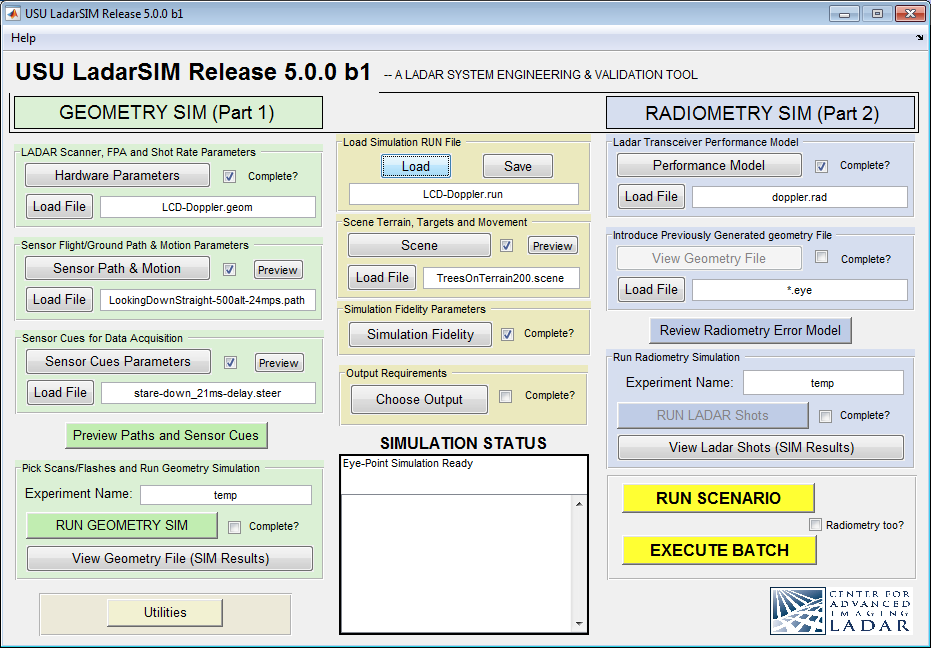
\includegraphics[width=.8\columnwidth]{figs/LadarSIM}
	\vspace{1em}
	\caption{Main GUI for running LadarSIM.}
	\label{fig:LadarSIM}
\end{figure}

The green section on the left side of the GUI is the geometry simulation. This section simulates
the scenario from a strictly geometric stand point. This simulation produces a point cloud using 
the scanner parameters, sensor flight path, and scene. The geometric simulation runs independently
of the type of lidar to be simulated. The geometric measurements generated by the geometry simulation
are used when LadarSIM simulates the actual performance of the specified lidar system. 

The blue section on the right side of the GUI is the radiometric simulation. Again this cannot be run
until after a geometric simulation of the scenario has been run. This side of the of the GUI can be used
to simulate the performance of a particular lidar configuration. Parameters relating to the optical efficiency, 
transmitted beam, receiver, and range processing can be customized. The purpose of separating the geometric 
and radiometric simulations is that the output of a single geometric simulation can be used to evaluate the 
performance of different lidar configurations. 

\section{Geometry Simulation Modification}
The geometry simulation produces two useful items. The first is a point cloud of the scenario based only on the
flight path, scanning parameters, and the scene. The second is what is called the "eyepoint file." This file 
contains measurements of the true range for each instance that the lidar would take a measurement based on the
scanning parameters. This file can be saved for later use or passed directly to the radiometry simulation. 

Before a simulation of Doppler lidar was added to LadarSIM only time of flight (TOF) lidar was supported. In time of
flight lidar no direct measurement of velocity is taken so it was not necessary to include true measurements of 
radial velocity. The measure of radial velocity is, however, crucial to the simulation of a Doppler lidar system.
For this reason the geometry simulation was modified to add radial velocity measurements to the eyepoint file. 

\section{Radiometry Simulation Modification}
Because the transmit and receive processes are very different for TOF and FMCW lidar, more modification
was necessary to the simulation of the radiometry simulation. Figure \ref{fig:radParam} shows the "performance model"
window. This is where parameters pertaining to the radiometry simulation are set. LadarSIM divides these parameters into
four sections, optics, transmitter, receiver, and range processing. The parameters in these subcategories are different 
for TOF and FMCW lidar, the radio button pair marked "Instrument Type" selects which type of system to be customized. 
\begin{figure}[!htb]
	\centering
	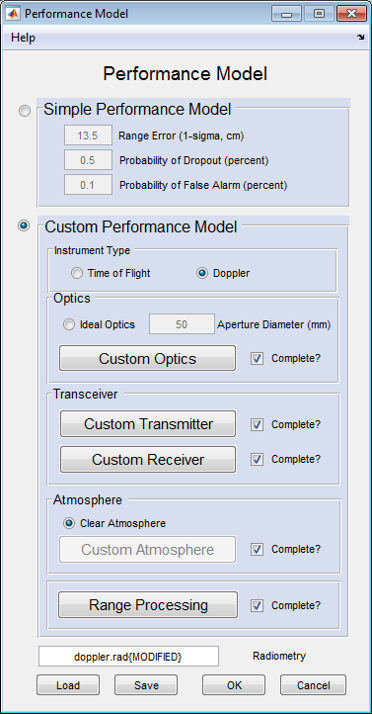
\includegraphics[width=.5\columnwidth]{figs/radParamGUI}
	\vspace{1em}
	\caption{Radiometry parameter GUI.}
	\label{fig:radParam}
\end{figure}  

The Custom Optics GUI shown in figure \ref{fig:opticsGUI} allows the user to specify the optical efficiency of the transmitter
and receiver, the aperture diameter, and detector fill factor. These parameters are common between TOF and FMCW lidar so this 
GUI is used for both. 
\begin{figure}[!htb]
	\centering
	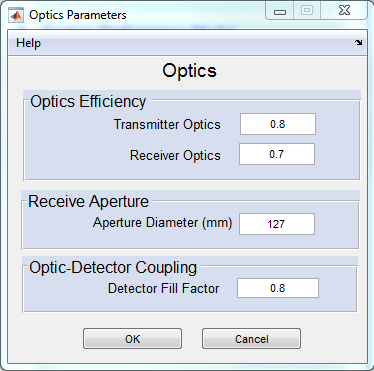
\includegraphics[width=.6\columnwidth]{figs/opticsGUI}
	\vspace{1em}
	\caption{Optical parameters GUI.}
	\label{fig:opticsGUI}
\end{figure}  

The Doppler Transmitter GUI is shown in figure \ref{fig:dopTXGUI}. The user can use this GUI to set parameters related to 
the transmitted laser. Beam divergence, laser wavelength, and laser line width are important characteristics of the laser that 
have a large effect on the performance of the system. The "Temporal Pulse Shape" box allows users to specify the laser power and 
the chirp shape, which has a direct effect on the capabilities of the system. Chirp bandwidth length in time have a
direct impact on the maximum resolution the system will be capable of.  
\begin{figure}[!htb]
	\centering
	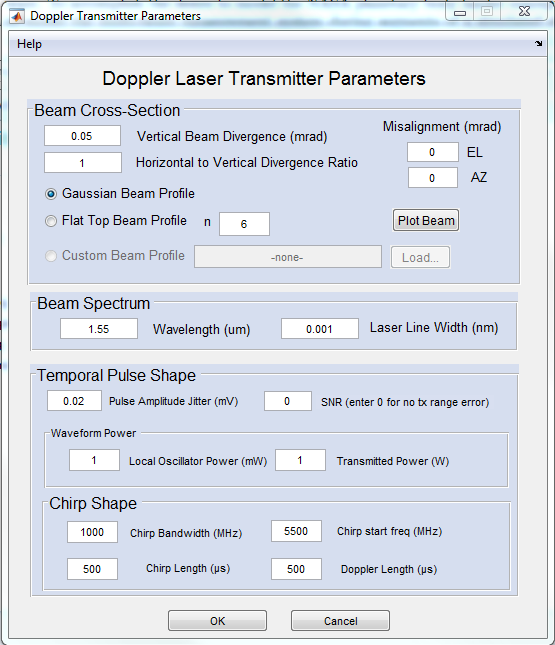
\includegraphics[width=.6\columnwidth]{figs/dopTxGUI}
	\vspace{1em}
	\caption{Transmitter parameters GUI.}
	\label{fig:dopTXGUI}
\end{figure}  

The "Receiver Parameters" GUI can be used to describe the electronics of the receiver. The behavior of the photo-diode is important 
because it's bandwidth is leveraged in the directly by the homodyne self-chirped detection architecture discussed in section \ref{sec:homodyneSelf}. The gain and bandwidth of other analog receiver electronics can also be specified in this GUI. 
\begin{figure}[!htb]
	\centering
	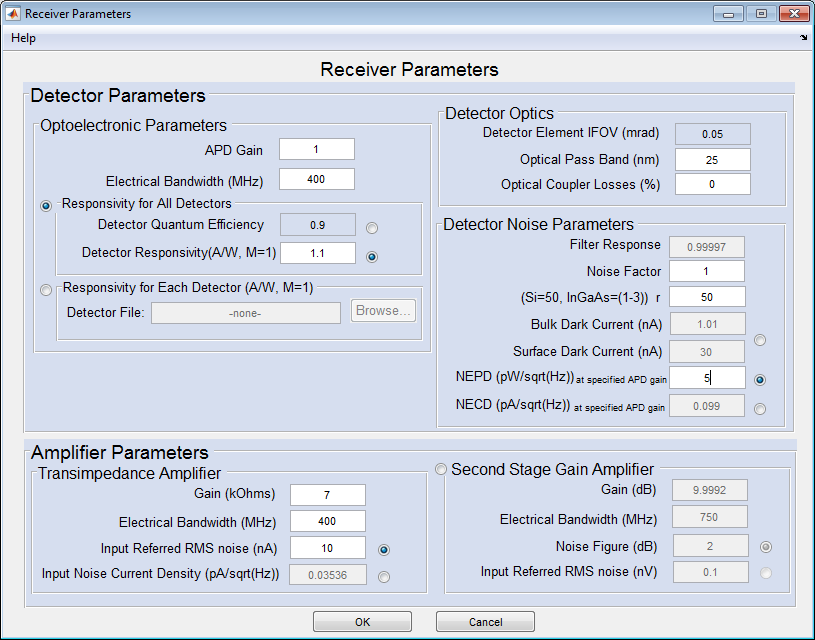
\includegraphics[width=.8\columnwidth]{figs/RxParamGUI}
	\vspace{1em}
	\caption{Receiver parameters GUI.}
	\label{fig:dopRXGUI}
\end{figure} 

Parameters directly related to range processing are set in the "Doppler Range Processing" GUI shown in figure \ref{fig:radParam}. The 
threshold to noise ratio (TNR) dictates where the detection threshold should be set in relation to the noise and effects the probability
of detection and false alarm. The maximum range and Doppler velocity the system is capable of resolving is dependent on the sample rate. 
The user can select to specify either the maximum  
\begin{figure}[!htb]
	\centering
	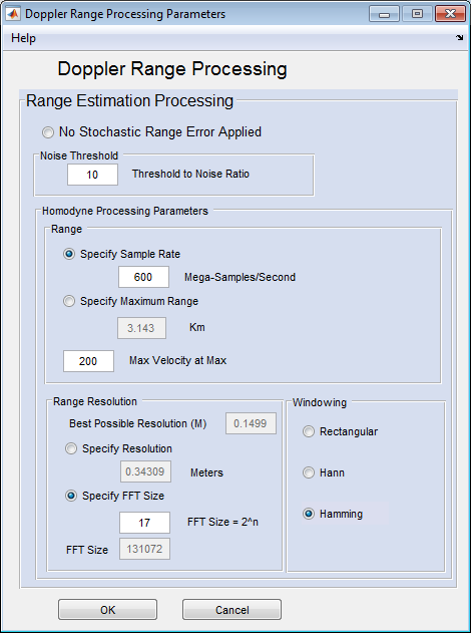
\includegraphics[width=.8\columnwidth]{figs/rangeParamGUI}
	\vspace{1em}
	\caption{Range processing parameters GUI.}
	\label{fig:rangeGUI}
\end{figure} 
